%
% $RCSfile: ontology.tex,v $
%
% Copyright (c) 2001-2004. Christian Heller. All rights reserved.
%
% No copying, altering, distribution or any other actions concerning this
% document, except after explicit permission by the author!
% At some later point in time, this document is planned to be put under
% the GNU FDL license. For now, _everything_ is _restricted_ by the author.
%
% http://www.cybop.net
% - Cybernetics Oriented Programming -
%
% http://www.resmedicinae.org
% - Information in Medicine -
%
% @author Christian Heller <christian.heller@tuxtax.de>
%

\subsection{Ontology}
\label{ontology_heading}

Manifold definitions of the word \emph{Ontology} exist. They come from philosophy,
metaphysics, information technology and others -- too many to list here.
This document uses its own, adapted definition and considers an ontology to be
\emph{a strict hierarchy of abstract items, organized in levels of growing
granularity, that are solely unidirectionally related}. It such represents a
systematic description of complex domain contexts.

\begin{figure}[ht]
    \begin{center}
        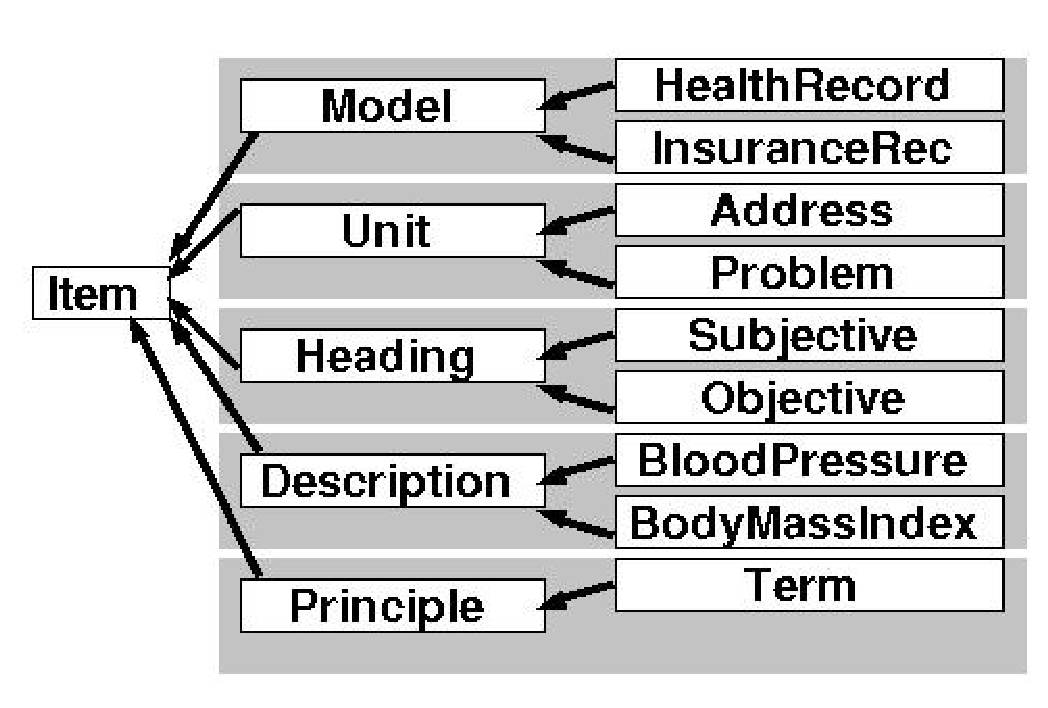
\includegraphics[scale=0.4]{vector/electronic_health_record_ontology.eps}
        \caption{Electronic Health Record Ontology}
        \label{electronic_health_record_ontology_figure}
    \end{center}
\end{figure}

Figure \ref{electronic_health_record_ontology_figure} shows one possible ontology
of an electronic health record, as described in the previous section.

